\section{Existing verification tools}
Software unit testing can be achieved by almost any tool.  The choice
of verification tool is therefore not the most interesting when it
comes to pure unit testing. One can of course take the simplicity to
achieve good unit testing into account, but it is not what makes a
verification tool unique for this projects goals.

%% TODO: �r det inte en del av Avgr�nsningarna och inte Metodik?
Since the purpose is about benchmarking software the phase
``verification of software safety requirements'' will not influence
the choice. To be able to test this phase, a greater amount of
components of the whole system must be available. Such components
include hardware, and this report will not cover hardware
integration. The implementation should be able to run on a standard
PC-machine.

The most interesting part of the V-model is the phase ``software
integration and testing''. Is there a tool that can be used to easily
combine tests and requirements from different modules? Is it possible
to test functional safety concept from this combination, for example
by corrupting some software elements?

Two tools that can be used in order to achieve better code and some
functional safety is SPIN and Parasoft C/C++test. While SPIN can
verify the model, Parasoft C/C++test defines policies on work flow as
well as coding.

\subsection{SPIN}
SPIN is used to trace logical design errors in distributed software
\cite{SPIN:manual}. It supports a high level language, called Promela,
to specify system descriptions. Promela is an acronym for PROcess MEta
LAnguage, and is a verification model language. The system properties
that should be checked are written in logical temporal language
(LTL), and SPIN reports errors such as deadlocks, race conditions and
incompleteness between these properties and the system model. It also
supports embedded C code as part of the model specifications. It
supports random, interactive and guided simulation, with both partial
and exhaustive proof techniques.

\subsection{Parasoft C/C++test}
Parasoft C/C++test is a commercial integrated development testing
solution for C and C++ \cite{PARASOFT:datasheet}. It automates code
analysis, and enforces code policies depending on given rules. The
solution is part software, part practical rules for team
collaboration.  It can detect certain runtime errors such as memory
access errors, null pointer referencing, buffer overflows, division by
zero and the use of uninitialized memory or variables. It can create
and execute unit tests and collect code coverage from application
executions.

Parasoft claims that it should be possible to satisfy some of the ASIL
requirements using their solution \cite{PARASOFT:ASIL}.

\section{Specification}
In AUTOSAR, specifications for each module is given in text
form. Therefore before a module can be tested, that specification must
first be implemented in code.

\section{Testing}
Properties of a module have to take the current state in
consideration, since most functions written in an imperative language
are not immutable. This gives raise to the idea of a state based
testing tool.

\section{Choice of AUTOSAR module to test}
%% TODO: "less complicated" in what way?
When deciding which AUTOSAR module to test, there were a number of
modules up for discussion. Since the goal was to get a proof of
concept; examining if it was possible to get an ASIL-classification
and achieve functional safety using QuickCheck, it seemed preferable
to choose a less complicated module. It was also desirable to have the
actual C code and not just library files, because then we could check
ambiguities in AUTOSAR in a more efficient way.

\section{Implementation}
The module that was chosen, was already unit tested and run actively
in lab environment.

%% TODO: eventuellt skriva om delar i stycket, framf�r allt i slutet.
The implementation of the properties was done to be able to test API
calls, also described in appendix~\ref{APP:QUICKCHECK}, against the
C-code. QuickCheck then checked that the postconditions held,
according to figure \ref{FIG:api_calls}. The postconditions were
written to test that AUTOSAR requirements held. In other words that
the API calls were called correctly.

\begin{figure}[!ht]
  \begin{center}
    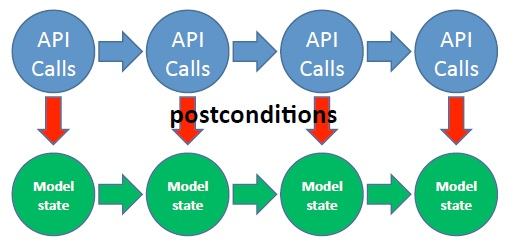
\includegraphics{pictures/api_calls.jpg}
  \end{center}
  \caption{Shows Erlang modeled states with calls against the C-code}
  \label{FIG:api_calls}
\end{figure}

\subsection{Formal Notation}
For QuickCheck to be able to automatically generate test cases,
AUTOSAR specifications written in a natural language, needed to be
transformed into properties in Erlang code. In other words
transforming informal notation into formal notation.

A problem when translating the AUTOSAR specifications into code was
that there were ambiguities. It was easy to see that there were room
for different interpretations, which most likely would result in
errors later. This is described more precise in section
\ref{SUBSEC:CONFLICTS}.

The translating process was done iteratively as described in section
\ref{SEC:ITERATIVE}.

\subsection{Independence of the Erlang implementation}
The implementation in Erlang was done independent from the design
choices in the C-code. The idea was to ensure an independent model; if
the model was inspired by the C-code, it could have transmitted
faults. Implementing the Erlang module independent of the
C-implementation would also result in that ambigousities in the
AUTOSAR specification would be easier to find. This since two
different interpretation of the same specification would eventually be
available.

\subsection{Iterative strategy}
\label{SEC:ITERATIVE}
The implementation of the AUTOSAR module in Erlang was done in an
iterative way. Every piece of code were not required to be implemented
before tests could be run. This is because a module in AUTOSAR consist
of a number of API calls. It was enough to implement some of the
specifications for one API call before tests could be run. Of course
this tested only the implemented part of the C-code. Early tests may
not have fully tested the implemented API call because some branches
in the C-code will never have been reached before other unimplemented
API calls.

\subsection{Conflicts and Bugs}
\label{SUBSEC:CONFLICTS}
%% TODO: Skriv om stycket "every programmer makes mistakes". Det borde
%% isf l�ggas till om ambiguites i AUTOSAR tidigare.
Early in the implementation phase QuickCheck found differences between
the Erlang and C-implementation. This was expected because every
programmer makes mistakes.  The question was whether the fault was in
the C-code or the Erlang code. Then the API was thoroughly read and a
conclusion was made based on this. Either a bug in the C-code was
found or the Erlang-code needed to be corrected. There were however
cases when the API was ambiguous. In those cases the C-interpretation
was chosen as correct and the ambiguous specification written down.

Bugs in the C-code was found early, even though it already run
actively in lab environments.

If a bug in the C-code was discovered how should the work be
continued? Since QuickCheck terminates as soon as it finds a counter
example, a method for resolving conflicts was needed to be able to run
further tests. Some alternatives were discussed.

\begin{enumerate}
  \item Fix the C-code, in other words change the source
    code. Knowledge about the structure in the C code is needed.
    \label{ENUMERATE:FixCCode}
  \item Mocking, in other words simulate different C code output. The
    pitfall is if that each mocked function eliminates all bugs in the
    function. Not only a selected subset; at most one bug per function
    can then be found.
  \item Change the Erlang module to a faulty behavior to follow the C
    implementation. The problem is that other configurations or
    updated versions of the C code will show up as faulty when using
    the same Erlang model.
\end{enumerate}

Item \ref{ENUMERATE:FixCCode} was chosen because this was the most dynamic
and allowed further bugs to be found, see section \ref{sec:handlebugs}.

When thoroughly reading the AUTOSAR API not only ambiguous rules were
found but also rules that contradicted each other were recognized. In
those cases the implementation in the C-code was followed.

\subsection{Advantage of having the Actual C-code}
%% TODO: Sista meningen lite l�sryckt?
When it did not exist a clear interpretation of the AUTOSAR
specification, a great method for understanding, was to examine the C
code. Even though QuickCheck can be used to test libraries when the source code is not available.

\section{Implementation structure}
The final implementation consisted of several Erlang modules. Table
\ref{TABLE:MODULES} lists the modules defining the watchdog manager.
There are also other modules that reads configuration files, defines the
generators, measuring code coverage etcetera, those modules have however no
equivalence in the C-code.

\begin{table}[!ht]
\caption{Erlang modules defining the watchdog manager}
\label{TABLE:MODULES}
\begin{tabular}{l|p{0.7\linewidth}}
\hline
modules & descriptions \\
\hline
wdgm\_helper            & Helper module used by  wdgm\_helper \\
wdgm\_checkpointreached & Erlang version of checkpointreached, see \ref{SEC:CHECKPOINTREACHED} \\
wdgm\_main              & Erlang version of the main function, see \ref{SEC:MAINFUNCTION} \\
wdgm\_pre               & Checks for AUTOSAR preconditions \\
wdgm\_post              & Checks for AUTOSAR postconditions \\
wdgm\_next              & Defines the watchdog manager model, uses
wdgm\_checkpointreached, wdgm\_main and wdgm\_helper
\end{tabular}
\end{table}

\section{Evaluation of the Implementation}
If tests come back positive, it does not really say much more than
that those tests evaluated to true. There is a need to evaluate what
was actually tested.

\subsection{Verifying the tests}
When the module was fully implemented in Erlang code there had to be
some assurance of that every piece of code in the C implementation was
actually tested.  Code coverage for the Erlang implementation was
measured using the Erlang module \emph{cover}. The coverage were only measured
on the modules listed in \ref{TABLE:MODULES} since they are the only modules
that defines the Erlang version of the watchdog manager.

To be able to measure
the code coverage of the C-code the commercial tool Bullseye Coverage
was used. When using those tools it was easy to see that the result
was not good enough. The main problem seemed to be that the WdgM was
put in an absorbing state and because of that the following commands
interesting; they did not change the state. The reason for that an
absorbing state was reached was the availing of negative testing. The
testing was negative because invalid command sequences and arguments
were generated.

Figure \ref{FIG:ONERUN} shows an example of how the status of the
watchdog manager changed during the execution of API calls. After a
number of commands the absorbing state \emph{stopped} was reached.

\begin{figure}
  \begin{center}
    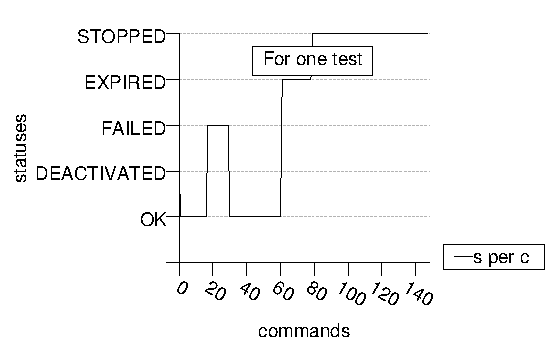
\includegraphics{generated_pictures/one_test_history_statuses_freescale.pdf}
    \caption{Shows changes to the global status in the execution of one QuickCheck test.}
    \label{FIG:ONERUN}
  \end{center}
\end{figure}

\subsection{Finding better test cases}
The next step was to tweak the generators that were used by QuickCheck
to construct valid API-calls. This is done to find better test cases,
i.e. there were a number of branches in the C-code that needed a
specific sequence of API calls with correct arguments, to be
reached. For example, it is unreasonable to test functions often when
the initialization function \lstinline!WdgM_Init! has not yet been
called.

Thanks to QuickCheck's weight feature, it is simple to change the
ratio of the generation of certain API calls; by matching the state
and the function name of the API call, one can change the probability
of generation of that call.

As an example we have the initialization function
\lstinline!WdgM_Init!  were we want to have a high priority if it has
not been called yet, and a low priority if it has been called
previously.
\begin{lstlisting}
weight(S,  'WdgM_Init') ->
  case S#state.initialized of
    true                           -> 1;
    _                              -> 200
  end;
\end{lstlisting}
It is a good idea not to lower some ratios to much, because then
certain API sequences would not be generated, and bugs might be
missed.

The tweaking of the generators were implemented in a iterative way by
changing the probability properties of the generators and analyze the
results and the coverage. After the analysis, the generators were
tweaked even more to make the result and coverage even better.

To get a better picture of the work flow used in this thesis see
figure \ref{fig:workflow}.

\begin{figure}[!ht]
  \caption{Work flow}
  \label{fig:workflow}
  \fbox{
    \parbox{\linewidth}{
      \begin{enumerate}
      \item Construct a model for an AUTOSAR module in Erlang
      \item Run QuickCheck for this model and compare the results with the output from
        the C code. \label{compare}
      \item Tweak the generators for the test cases \label{generators}
      \item Evaluate the results
        \begin{enumerate}
        \item Evaluate the state space
        \item Evaluate if the test cases are relevant
        \item Collapse irrelevant states
        \end{enumerate}
      \item Are the results good enough, does it satisfy the requirements for the ASIL
        levels?
      \item If not go the step \ref{compare}
      \end{enumerate}
    }}
\end{figure}

A challenging step is the analysis of the results. If the testing tool
returns zero errors what does that say about the robustness of the
input byte code? Passed 100 of 100 tests is just a statement and does
not say anything more than that some tests passed. Can tests be
implemented in a clever way so that it is possible to get some kind of
confidence on the correctness of the code?

\section{Configurations}
When the code coverage was calculated it was recognized that every
piece of code wasn't executed. The reason seemed to be that the
current configuration disallowed the execution of some parts of the
code, even though the program behaved correctly. It was easy to run
tests on several configurations, because the implementation of the
Erlang module was made independent of configurations. This resulted in
almost full coverage.

Three configurations with different complexity was used. The first
one, an example configuration (this will further on be called the
Example configuration), had many supervision functions configured for
each mode, and followed a strict execution of the program.

There were also a minimal configuration (BSI configuration) which, in
lack of supervision functions, only could change the global status
between \lstinline!WDGM_GLOBAL_STATUS_OK! and
\lstinline!WDGM_GLOBAL_STATUS_DEACTIVATED!. This on the other hand,
tested some null conditions, for example when there are no supervised
entities.

The last configuration (named Freescale configuration), which was one
of the configurations that were used actively in lab equipment, was
similar to the example configuration but a bit more relaxed. The
global status stayed in a non-absorbing state more often; it was
easier to do positive testing.

%% TODO: St�mmer sista meningen? St�mmer referensen.?
The tweaking of generators, where the aim is to generate better test
cases, seemed in some sense to be configuration dependent. Better test
cases were generated if the generators were tweaked according to a
specific configuration, see chapter \ref{CHAPTER:RESULTS}.

\section{Calling the API commands}
\label{SEC:CALLING_COMMANDS}
API calls were executed by QuickCheck using the \emph{run\_commands/1}
function according to appendix \ref{SEC:QuickCheckIntro}. The runtime
environment module (RTE) is however responsible for the scheduling of
the main function, which according to AUTOSAR, should be executed in a
given time interval. Since the RTE was not available when testing the
watchdog manager the main function was called randomly and it was
assumed that every time the main function was called a given amount of
time had passed.

Except for the main function, only one internal algorithm that was
used by the watchdog manager was time dependent, namely the deadline
supervision algorithm. A supervised entity with deadline supervision
consists of two checkpoints. One start checkpoint, one stop checkpoint
and a maximum time it should take to reach the stop checkpoint after
the start checkpoint was reached. The AUTOSAR specification was
however lacking of a clear definition of how time should be
handled. The C code just used ticks, not actual time stamps, which
was incremented every time the main function was called. It was in
other words assumed that the RTE was able to execute the main function
correctly and a fixed amount of ticks would always represent the same
amount of time. Accepting this solution it was easy to adopt the same
approach in the Erlang module. More about this can be found in section
\ref{SEC:FUNCTIONAL_SAFETY_TIME}.

\section{Model State}
The model state was constructed as minimal as possible. Even though it
was tempting to use a more efficient data structure, a simple Erlang
record was used to represent the model state. Using more efficient
data structures could for instance speed up the execution of
tests. The main reason for using a record was to make it easy to
follow the model state when using \emph{eqc\_statem:show\_states/1},
see appendix \ref{APP:QUICKCHECK}. The efficiency of the test model
was considered less relevant than the readability of the model state.
The idea was to make it easy to find the actual bug, when conflicts
arouse between the C-code and the Erlang module. Running the actual
tests was also not considered time or memory critical.
